\documentclass[10pt,onecolumn,a4paper]{article}
\usepackage{epsfig,graphicx,subfigure,amsthm,amsmath}
\usepackage[font=tiny,labelfont=bf]{caption}
\usepackage[top=15mm, bottom=15mm, left=15mm, right=18mm]{geometry}
\usepackage{color,xcolor}
\usepackage{authblk}
\usepackage{multicol}
\usepackage{bidipoem}
\usepackage[linktocpage=true,colorlinks,citecolor=blue,pagebackref=true]{hyperref}
\usepackage{xepersian}
\settextfont[Scale=1.2]{A Mashin Tahrir}
\setlatintextfont[Scale=1]{Courier New Bold}
\setcounter{Maxaffil}{0}
\renewcommand\Authands{ و }
\renewcommand\Authand{ و }

\begin{document}
    \title{عنوان این مستند}
    \author[1]{نویسنده اول}
    \author[2]{نویسنده دوم}
    \affil[1]{وابستگی اول \lr{Affiliation 1}}
    \affil[2]{وابستگی دوم \lr{Affiliation 2}}
    \date{۲ تیر ۱۳۸۱}
    \maketitle

    \section{}
    یک بخش با شماره بدون عنوان\\
    خط بعدی \lr{Next line} بعد از خط اول
    
    \LTR\noindent\lr{
    An English sentence here
    }\RTL

    \section{بخش دوم}
    یک بخش با شماره با عنوان   
    \paragraph{اول}
    یک پاراگراف با عنوان    
    
    \paragraph{}
    یک پاراگراف بدون عنوان با تورفتگی در خط اول\\
    خط دوم همراه با یک \textit{یک متن ایتالیک}.
    
    \par\noindent
    یک پاراگراف بدون تورفتگی و بدون فاصله با پاراگراف قبلی\\
    خط دوم پاراگراف

    \section*{}
    یک بخش بدون شماره بدون عنوان

    \section*{بخش چهارم}
    یک بخش بدون شماره با عنوان    

    % نمونه شعر کلاسیک فارسی
    \begin{center}
        به نام خداوند هستی بخش\\
        \bigskip

        \renewcommand\poemcolsepskip{2.0cm}
        \begin{traditionalpoem*}
            اَلا یا اَیُّهَا السّاقی اَدِرْ کَأسَاً\footnote{پاورقی} و ناوِلْها & اَلا یا اَیُّهَا السّاقی اَدِرْ کَأسَاً و ناوِلْها
            مرا در منزلِ جانان چه امنِ عیش چون هر دَم & جَرَس فریاد می‌دارد که بَربندید مَحمِل‌ها
        \end{traditionalpoem*}
    \end{center}

    % نمونه شعر نو فارسی
    \renewcommand\poemcolsepskip{0.5cm}
    \begin{modernpoem*}
        من از نهایت شب حرف میزنم\LTRfootnote{\lr{English footnote}}
        من از نهایت تاریکی
        و از نهایت شب حرف میزنم

        اگر به خانۀ من آمدی برای من ای مهربان چراغ بیاور
        و یک دریچه که از آن
        به ازدحام کوچۀ خوشبخت بنگرم
    \end{modernpoem*}

     % افزودن عکس به متن با عنوان
    \begin{figure}[htbp]
        \centering
        \makebox[\textwidth]{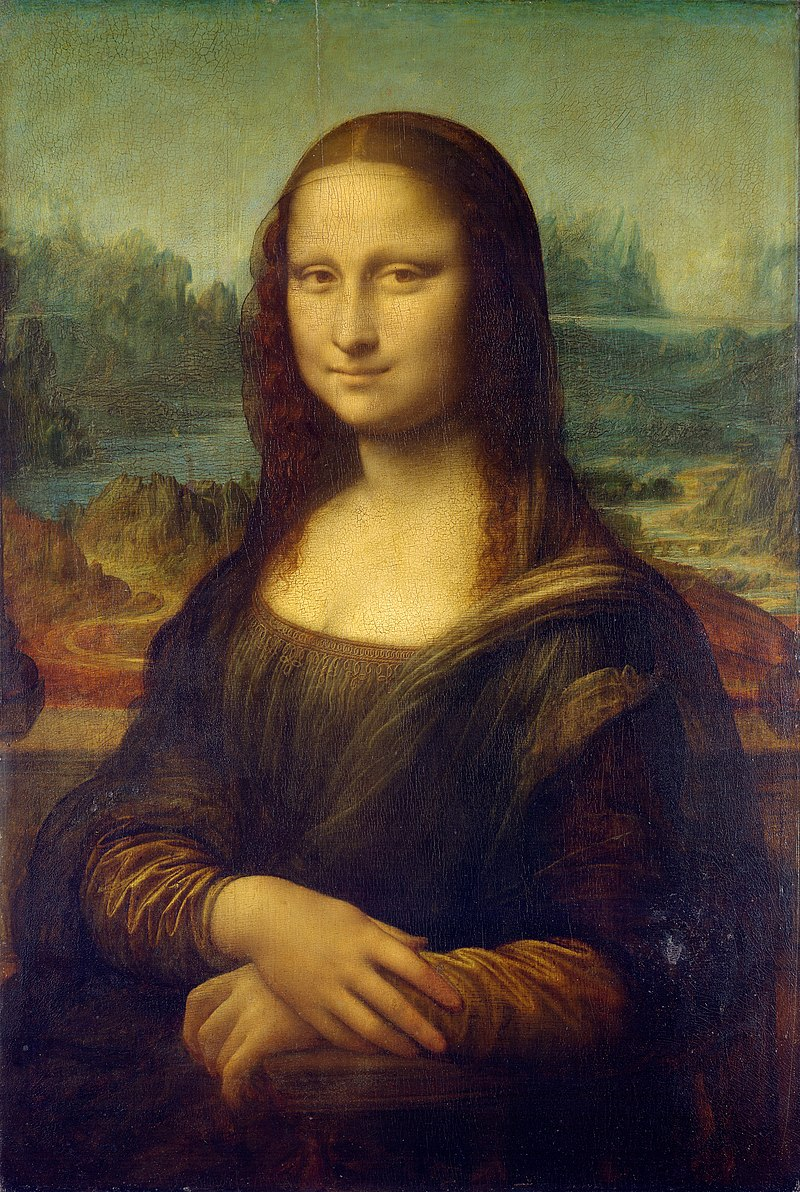
\includegraphics[keepaspectratio,width=0.4\textwidth,height=0.4\textheight]{Mona_Lisa.jpg}}
        \caption*{\lr{Mona Lisa - Leonardo da Vinci}}
        \label{fig:1}
    \end{figure}

    % افزودن عکس به متن
    \begin{center}
        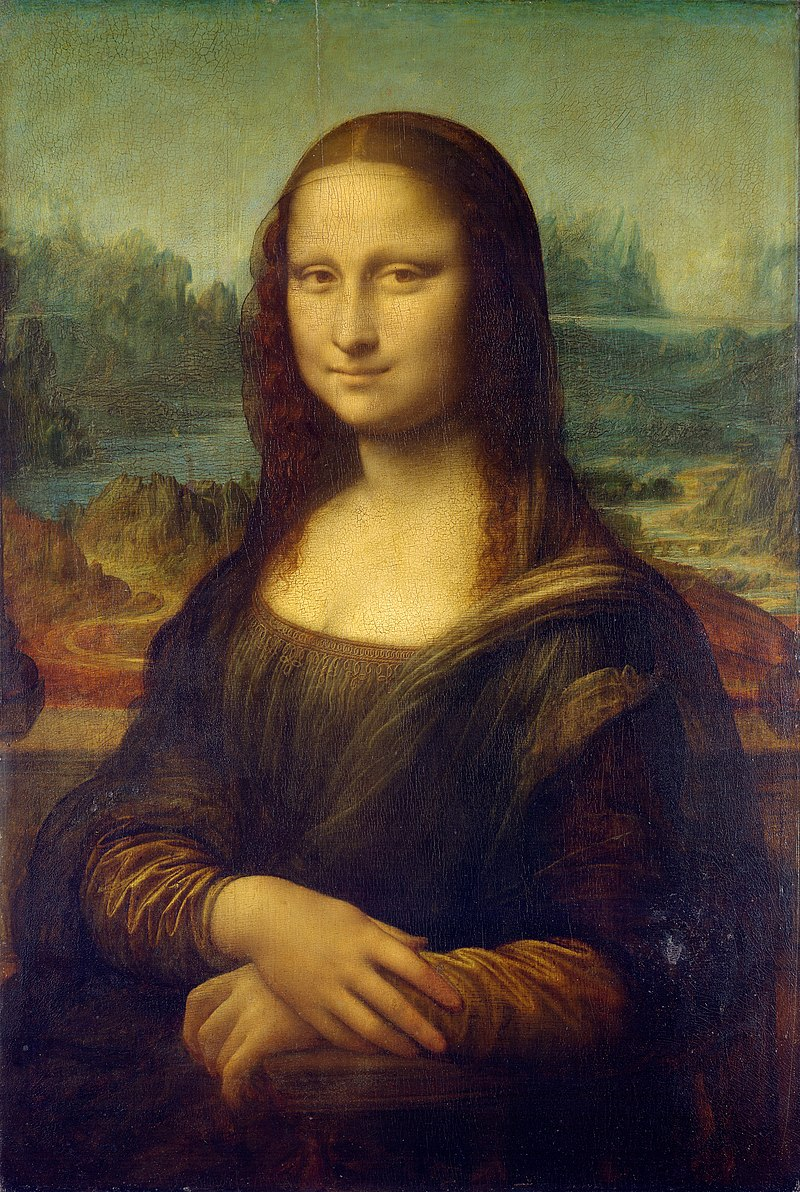
\includegraphics[keepaspectratio,width=0.4\textwidth,height=0.4\textheight]{Mona_Lisa.jpg}
    \end{center}

    \begin{flushleft}
        یک متن قرار گرفته در سمت چپ مستند\\
        \smallskip
        \date{6 آبان 1387}
    \end{flushleft}
\end{document}